
\chapter{Einleitung}

% Without it being a section, it fits on one page
%\section{Motivation}
Der Begriff \enquote{autonomes Fahren} hat spätestens seit den Autos von Tesla einen allgemeinen Bekanntheitsgrad erreicht. Damit ein Auto selbstständig fahren kann, müssen erst viele Hürden gemeistert werden.
Dazu gehört zum Beispiel das Spur halten, das richtige Interpretieren von Verkehrsschildern und das Navigieren durch komplexe Kreuzungen.

Bevor ein autonomes Fahrzeug Entscheidungen treffen kann, benötigt es ein möglichst genaues Modell seines Umfelds.
Hierzu werden von verschiedenen Sensoren wie Front-, Rück- und Seitenkameras und Abstandssensoren Informationen gesammelt und ausgewertet.
Aber vielleicht kann ein Auto nicht immer selbständig genügend Informationen zu seinem Umfeld sammeln? %\todo{(huhuhu Server implied huhuhu)}
%Diese Arbeit beschäftigt sich mit genau dem Thema, einem selbst fahrendem Auto Informationen zu anderen Teilnehmern an einer Kreuzung zu vermitteln.

Externe Sensorik könnte Informationen liefern, die das Auto selbst nicht erfassen kann.
Ein viel zu schneller Radfahrer hinter einer Hecke in einer unübersichtlicher Kreuzung?
Eine Lücke zwischen Autos, die ausreichend groß ist, um einzufahren ohne zu bremsen?
Die nächste Ampel wird bei Ankunft rot sein, ein schnelles und Umwelt belastendes Anfahren ist nicht nötig?
Ideen gibt es zuhauf.

Aber was ist, wenn das System aussetzt?
Die Antwort hierzu ist einfach: das Auto muss immer noch selbstständig agieren können, externe Systeme sollen nur optionale Helfer sein.
Viel schlimmer ist es dagegen, wenn das unterstützende System falsche Informationen liefert.
Eine Lücke zwischen Autos, wo keine ist; eine freie Fahrbahn, wo ein Radfahrer fährt; ein angeblich entgegenkommendes Auto, eine unnötig Vollbremsung, ein Auffahrunfall.
Ein solches System muss sicher sein -- nicht nur vor Hackern.
Es muss funktional sicher sein, Redundanzen und Notfallsysteme müssen jederzeit greifen.

Aber was nützt die beste Idee, die ausgeklügelte Strategie, wenn nur ein einziges Mal vergessen wurde, einen Rückgabewert auf den Fehlerfall zu prüfen?
Was nützt es, wenn Strategien für das Freigeben von Speicher in Notfallsituationen einen Sonderfall übersehen haben?
Das System handelt total unvorhersehbar.

Was wäre, wenn es eine Programmiersprache geben würde, die so etwas nicht zulässt: die fehlerhaften Strategien zur Compilezeit findet und die Compilation stoppt; die trotz erzwungener Sicherheitsmaßnahmen, schnell und echtzeitnah reagieren kann und sich nicht vor Geschwindigkeitsvergleichen mit etablierten, aber unsicheren Programmiersprachen, scheuen muss?

Diese Arbeit soll zeigen, dass Rust genau so eine Programmiersprache ist und sich für sicherheitsrelevante, hoch parallelisierte und echtzeitnahe Anwendungsfälle bestens eignet.
%Könnte Rust die Antwort sein? \todo{zuuu viele Fragen}



\clearpage % auch wenn julian sagt es ist behindert
\section{Projektkontext}
\begin{figure}[H]
	\label{test 123}
	\centering
	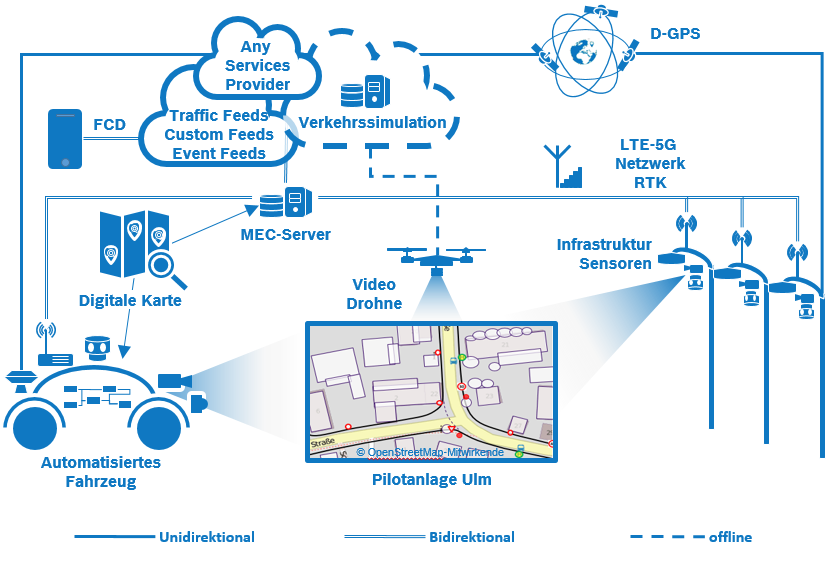
\includegraphics[width=\textwidth]{images/MECView_Arch_de_V1_mod.png}
	\caption[Übersicht über das Forschungsprojekt]{Übersicht über das Forschungsprojekt\protect\footnotemark}
\end{figure}
\footnotetext{Quelle: \url{https://www.uni-due.de/~hp0309/images/Arch_de_V1.png} (Legende verschoben)}

Diese Abschlussarbeit befasst sich mit dem Kommunikationsserver von \gls{mec}-View.
Das \gls{mec}-View Projekt wird durch das \gls{bmwi} gefördert und befasst sich mit der Thematik hochautomatisierter Fahrzeuge.
Es soll erforscht werden, ob und in wie weit eine durch externe Sensorik geleistete Unterstützung nötig und möglich ist, um in eine Vorfahrtstraße automatisiert einzufahren.

Das Forschungsprojekt ist dabei ein Zusammenschluss mehrerer Unternehmen mit unterschiedlichen Themengebieten.
Die IT-Designers Gruppe beschäftigt sich mit der Implementation des Kommunikationsservers, der auf der von Nokia zur Verfügung gestellten Infrastruktur im 5G Mobilfunk als \gls{mec} Server betrieben wird.
Erkannte Fahrzeuge und andere Verkehrsteilnehmer werden von den Sensoren von Osram via Mobilfunk an den Kommunikationsserver übertragen.
Der Kommunikationsserver stellt diese Informationen dem Fusionsalgorithmus der Universität Ulm zur Verfügung und leitet das daraus gewonnene Umfeldmodell an die hochautomatisierten Fahrzeuge der Robert Bosch GmbH  und der Universität Ulm weiter.
Durch hochgenaue, statische und dynamische Karten von TomTom und den Fahrstrategien von Daimler und der Universität Duisburg soll das Fahrzeug daraufhin automatisiert in die Kreuzung einfahren können.

%\subsection{Ablauf}
%Externe Sensoren übermitteln erkannte Fahrzeuge via Mobilfunk an einen \gls{mec}-Server, der direkt am Empfängerfunkmast angeschlossen ist. \todo{platform, vm?}
%Nachdem die erkannten Fahrzeuge der verschiedenen Sensoren zusammengeführt wurden (Fusionsalgorithmus), sollen sie an das autonom fahrende Fahrzeug über Mobilfunk übermittelt werden.
%Somit erhält das Fahrzeug bereits im Voraus Einsicht über eventuelle Möglichkeiten in die Vorfahrtsstraße einzufahren und könnte deshalb beispielsweise die Geschwindigkeit anpassen.
%Zudem sollen bei unübersichtlichen Kreuzungen somit zuverlässiger andere Verkehrsteilnehmer erkannt werden.


\section{Zielsetzung}

Zu dem zuvor beschriebenen Verhalten des Kommunikationsservers besteht bereits eine Implementation in C++.
%Dies ist aus Sicht der funktionalen Sicherheit (siehe \autoref{safety}) ein \todo{leidiges Thema}.
%Es besteht bereits eine Implementierung des Kommunikationsservers, die das zuvor beschriebene Verhalten umsetzt.
%Als Programmiersprache wurde C++ verwendet, ein aus funktionaler Sicherheit (siehe \autoref{safety}) betrachtetem Aspekt, \todo{leidiges Thema}.
Das Ziel dieser Bachelorarbeit ist es, eine alternative Implementierung des Kommunikationsservers in Rust zu schaffen.
Durch die Garantien (\autoref{rust:guarantees}) von Rust wird erhofft, dass der menschliche Faktor als Fehlerquelle gemindert und somit eine fehlertolerantere und sicherere Implementation geschaffen werden kann.

Eine Ähnlichkeit in Struktur und Architektur zu der bestehender C++ Implementation ist explizit nicht vonnöten.
Eventuelle Spracheigenheiten und einzigartige Features von Rust sollen im vollen Umfang genutzt werden können, ohne durch auferzwungene und unpassende Architekturmuster benachteiligt zu werden.
Es ist erwünscht, eine kompetitive Implementation in Rust zu schaffen.


\section{Aufbau der Arbeit}

Diese Arbeit ist im Wesentlichen in die folgenden Themengebiete aufgeteilt: Grundlagen, Anforderungs- und Systemanalyse, Systementwurf und Implementation und Auswertung.

Im Themengebiet Grundlagen sollen wesentliche Bestandteile dieser Arbeit erläutert und erklärt werden.
Hierzu zählt zum einen die Programmiersprache Rust in ihrer Entstehungsgeschichte, Garantien  und Sprachfeatures  (\autoref{rust}).
Zum anderen geht es um die hochperformante, serverbasierte Kommunikationsplattform mit ihren Protokollen (\autoref{com_plattform}) und dem Systemkontext, in dem diese betrieben wird.

In der Anforderungs- und Systemanalyse wird der Kontext, in dem der Server betrieben werden soll, genauer betrachtet. Umzusetzende funktionale und nicht-funktionale Anforderungen werden aufgestellt, sowie eine Übersicht über die Systeme gegeben, mit denen der Server interagiert wird.

Das Themengebiet Systementwurf und Implementation befasst sich mit dem theoretischen und praktischen Lösen der im vorherigen Kapitel aufgestellten Anforderungen. Aufgrund der Tatsache, dass es sich hierbei
um eine alternative Implementation handelt, wird zur bestehenden C++ Implementation Bezug genommen.
Architektonische Unterschiede im Systementwurf, die sich aufgrund von Sprach- und Bibliotheksunterschiede ergeben, werden hier genauer beschrieben.

Zuletzt wird eine Auswertung der Implementation aufgezeigt.

\todo{entsprechend zu aktualisieren}
